\part{Etude bibliographique}

\chapter{Apprentissage profond}

\section{Introduction}
L’apprentissage profond (\textit{deep learning} en anglais) est une branche de
l'intelligence artificielle (IA) qui s'intéresse à la résolution des problèmes
intuitifs, c'est-a-dire des tâches qui sont faciles à réaliser par les humains
mais difficiles à décrire formellement. Ce sont des problèmes qui semblent
automatiques, comme la reconnaissance des mots parlés ou des visages dans les
images. L'apprentissage profond permet aux ordinateurs d'apprendre des concepts
complexes en rassemblant de l'expérience. Cela permet d'éviter la spécification
formelle des connaissances dont l'ordinateur a besoin
	[\cite{Goodfellow-et-al-2016}].

\medskip
L'apprentissage profond utilise des réseaux de neurones profonds pour résoudre ces problèmes.
Ces réseaux sont des modèles computationnels qui imitent le fonctionnement
du cerveau humain [\cite{mcculloch_pitts_1943_nervous_activity}, \cite{rosenblatt_1958_perceptron}].
Ils sont constitués de plusieurs couches de neurones artificiels cachées qui traitent les données d'entrée.

\medskip
Il existe trois grandes catégories d'apprentissage automatique : \textit{supervisé}, \textit{non-supervisé} et \textit{semi-supervisé}. Dans l'apprentissage supervisé, on utilise un ensemble de données étiquetées, tandis que dans l'apprentissage non-supervisé, on ne dispose pas d'un ensemble de données étiquetées. L'apprentissage semi-supervisé est une combinaison d'apprentissage supervisé et non-supervisé. Dans l'apprentissage semi-supervisé, un ensemble de données est étiqueté, mais la majorité des données sont non étiquetées [\cite{Goodfellow-et-al-2016}, \cite{bishop_2016}].

\medskip
Dans l'apprentissage profond, plusieurs types d'architecture existent, chacune adaptée à des tâches spécifiques. Parmi les plus courants, on trouve: les \textit{réseaux de neurones convolutionnels} (CNN), les \textit{réseaux de neurones récurrents} (RNN), les \textit{réseaux de neurones générateurs adversaires} (GAN) et les \textit{réseaux de neurones de transformation} (Transformer) [\cite{Goodfellow-et-al-2016}].

\medskip
Dans ce chapitre, nous allons expliquer brièvement les différentes notions en relation avec l’apprentissage profond, telles que les couches du réseau, les fonctions d’activation, les types de réseaux, les connexions et les poids, le processus d’apprentissage et les types d’apprentissage.

\section{Réseau de neurones artificiels}
\label{sec:hotspot}
Un réseau de neurones artificiels (\textit{Artificial Neural Network} en anglais) est un modèle de traitement de l'information construit de couches de neurones interconnectées qui traitent les données d'entrée en les transmettant à travers des poids de connexion qui peuvent être ajustés par un processus d'apprentissage [\cite{aggarwal_2018}]. Ce réseau s'inspire du fonctionnement des neurones biologiques du cerveau.

\medskip
Chaque neurone dans les couches cachées du réseau reçoit des signaux d'entrée à partir des neurones précédents, les somme, et les transmet aux neurones de la couche suivante à travers une fonction d'activation. Les réseaux de neurones peuvent avoir plusieurs couches cachées, qui permettent de modéliser des relations non linéaires complexes entre les données d'entrée et de sortie. Ces réseaux neuronaux peuvent compter jusqu’à 150 couches, d'où le nom “profond”. [\cite{Goodfellow-et-al-2016}].

\medskip
Les réseaux de neurones peuvent faire des prédictions précises sur des données nouvelles qui ne sont pas vues pendant l'entraînement. Ils peuvent donc apprendre des relations complexes entre les données d'entrée et de sortie, ce qui leur permet de généraliser et de prédire les sorties pour de nouvelles données. Cependant, la qualité des prédictions dépend fortement de la qualité et de la quantité des données d'entraînement. Si les données d'entraînement sont mauvaises ou insuffisantes, les prédictions pour de nouvelles données peuvent être inexactes [\cite{Goodfellow-et-al-2016}].

\medskip
Les réseaux de neurones artificiels sont généralement caractérisés par:

\begin{itemize}
	\item \textbf{Traitement parallèle}: les réseaux de neurones sont capables d'effectuer plusieurs calculs simultanément. Cela les rend bien adaptés aux tâches nécessitant des calculs à grande échelle, telles que la reconnaissance d'images, la reconnaissance de la parole, et la traduction automatique [\cite{Goodfellow-et-al-2016}].
	\item \textbf{Apprentissage hiérarchique}: les modèles d'apprentissage profond sont généralement structurés en plusieurs couches . Chaque couche possède un niveau d'abstraction différent. Cela permet au modèle d'apprendre des motifs et des relations complexes dans les données, et plus le réseaux est profond, plus la capacité du modèle à découvrir ces relations est grande [\cite{Goodfellow-et-al-2016}].
	\item \textbf{Grandes quantités de données}: les modèles d'apprentissage profond nécessitent de grandes quantités de données pour s'entraîner efficacement. En effet, les modèles comportent un grand nombre de paramètres qui ne peuvent être réglés qu'à partir d'une grande quantité de données [\cite{Goodfellow-et-al-2016}].
\end{itemize}

\section{Connexions et poids}

Un réseau de neurones est constitué de nœuds et des connexions entre eux
	[\cite{aggarwal_2018}]. Chaque nœud possède un \textbf{ensemble d’entrées} (qui
sont souvent les sorties des nœuds de la couche précédente), un \textbf{poids}
et une valeur ajoutée appelée le \textbf{biais}. Dans les réseaux neuronaux, le
biais est un paramètre supplémentaire qui est ajouté à chaque neurone pour
ajuster sa sortie. Il permet au réseau de déplacer la fonction d'activation
horizontalement[\cite{Goodfellow-et-al-2016}].

\medskip
Lorsque des signaux entrent dans un neurones, chaque signal est multiplié par le poids associé à son entrée, puis additionné avec les autres résultats. Le biais est ensuite ajoute au résultat final et ce dernier est transmet vers les entrées des neurones de la couche suivante en passant par une fonction d'activation (voir la figure \ref{fig:fonctionnement-neurone}) [\cite{mcculloch_pitts_1943_nervous_activity}].

\medskip
On peut dire que la taille du réseau de neurones est définie par le nombre de ses paramètres et le nombre de ses couches, qui sont des variables appelées \textbf{hyperparamètres}. Par contre, les poids et le bais sont des paramètres entraînables. Au début de l'entraînement, on affecte à ces deux paramètres des valeurs aléatoires, et au fur et à mesure, les valeurs de ces deux paramètres sont ajustées et modifiées afin d'obtenir les bonnes valeurs [\cite{aggarwal_2018}, \cite{Goodfellow-et-al-2016}].

\section{Fonction d'activation}
Un neurone dans le réseau artificiel calcule la somme pondérée de ses entrées
et la valeur résultante de cette opération passe par une fonction appelée
\textbf{fonction d’activation} (ou \textbf{fonction de transfert}) avant d'être
transférée vers les neurones de la couche suivante. La sortie de neurone est
donc calculée selon la formule \ref{equ:activation-function}
[\cite{mcculloch_pitts_1943_nervous_activity}].

\newenvironment{conditions}
{\par\vspace{\abovedisplayskip}\noindent\begin{tabular}{>{$}l<{$} @{${}:{}$} l}}
		{\end{tabular}\par\vspace{\belowdisplayskip}}

\begin{equation}
	y=f\left(\sum_{i=1}^{n} w_ix_i + b\right)
	\label{equ:activation-function}
\end{equation}

Où:
\begin{conditions}
	w_{i}    &  le poids associé à l'entrée i \\
	x_{i}    &  la valeur associée à l'entrée i\\
	n &  le nombre total d'entrées  \\
	b &  le biais (constante entraînable ajoutée) \\
	f &  la fonction d'activation \\
	y &  la sortie du neurone \\

\end{conditions}

\begin{figure}[hbt!]
	\centering
	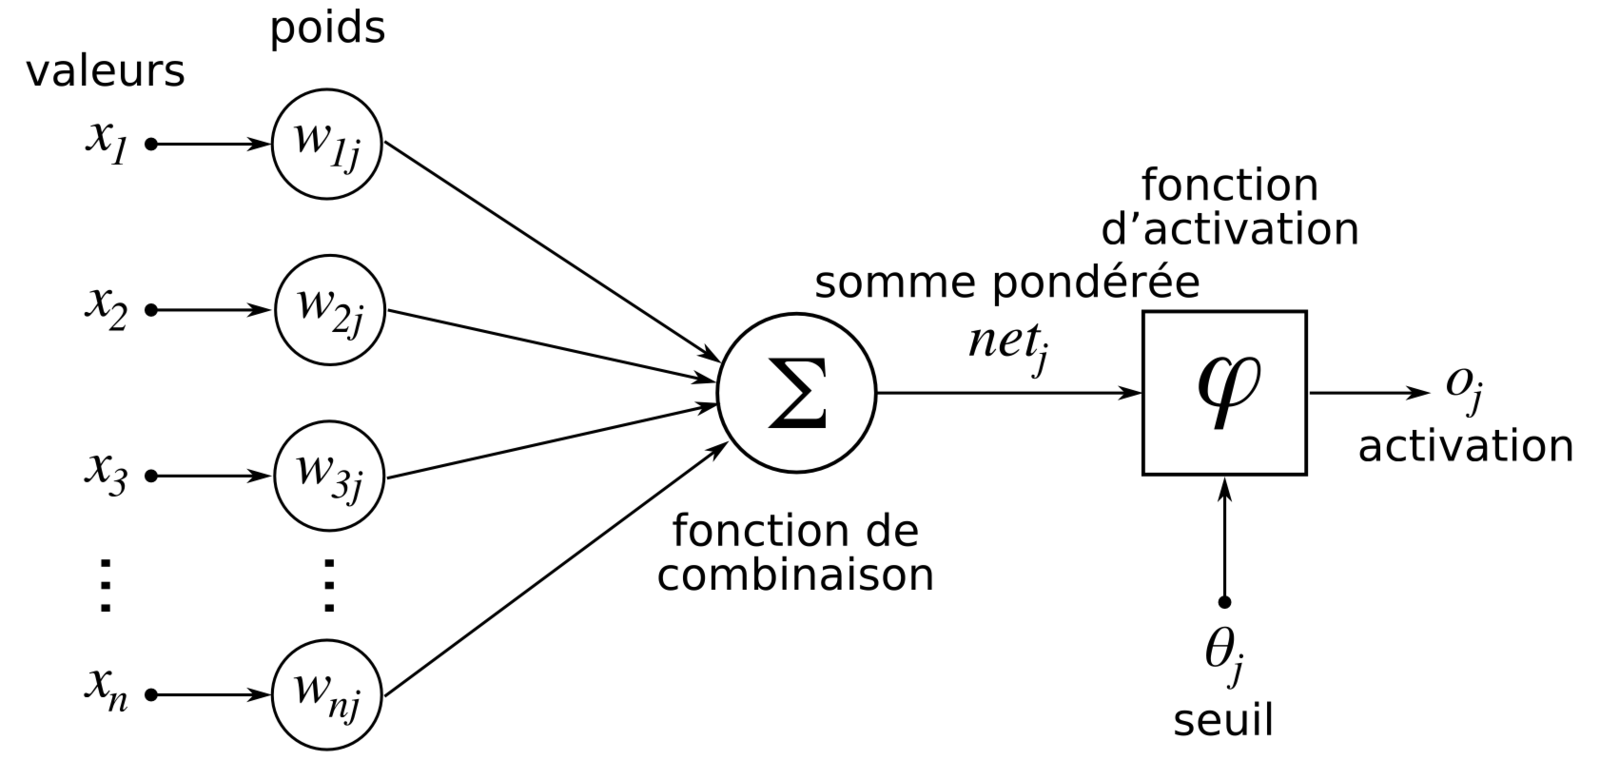
\includegraphics[width=10cm]{images_pfe/neurone.png}
	\caption{Le fonctionnement d'un neurone artificiel [\cite{mcculloch_pitts_1943_nervous_activity}].}
	\label{fig:fonctionnement-neurone}
\end{figure}
\FloatBarrier
\medskip

La fonction d'activation est utilisée pour introduire de la non-linéarité dans
le modèle, permettant ainsi de modéliser des relations complexes entre les
données d'entrée et de sortie [\cite{Goodfellow-et-al-2016}]. Les propriétés
d’une fonction d’activation doivent être vérifiées dans un problème
d'apprentissage profond. Ces propriétés sont:
\begin{itemize}
	\item \textbf{Non-linéarité}: lorsque la fonction d’activation est non linéaire, il est possible de prouver qu’un réseau neuronal à deux couches peut approximer n'importe quelle fonction continue sur un domaine compact à une précision arbitraire, ce que l’on appelle le \textbf{théorème d’approximation universelle} [\cite{Goodfellow-et-al-2016}].
	\item \textbf{L’intervalle}: lorsque l’intervalle des valeurs est fini, l'apprentissage de manière générale est plus efficace.
	\item \textbf{Différentiabilité}: cette propriété est importante quand les méthodes d’optimisation sont basées sur le gradient, car elles cherchent à optimiser l’apprentissage en se basant sur la  différentiabilité de la fonction.
	\item \textbf{Monotonie}: Une fonction d'activation est monotone si sa sortie augmente (ou diminue) à mesure que son entrée augmente. Cela garantit que le gradient de la fonction est toujours positif ou négatif, simplifiant ainsi l’apprentissage.
	\item \textbf{Efficacité en termes de calcul}: les fonctions d'activation doivent être efficaces en termes de calcul, afin que le réseau puisse être utilisé dans des applications en temps réel, sans ralentir le processus de l’apprentissage.
\end{itemize}
\medskip
Parmi les fonctions d'activation les plus couramment utilisées dans les réseaux de neurones, on peut citer:
\begin{itemize}
	\item \textbf{La fonction Sigmoïde}: si la probabilité d’un résultat est comprise entre 0 et 1, la fonction sigmoïde est le meilleur choix. Cette fonction est largement utilisée grâce à son intervalle et sa différentiabilité.
	      \begin{equation}
		      \sigma(x) = \frac{1}{1 + e^{-x}}
	      \end{equation}
	\item \textbf{La fonction Unité linéaire rectifiée (ReLU)}: c'est une fonction qui possède une dérivée et permet la rétropropagation (backpropagation) tout en étant efficace sur le plan informatique. Cependant, elle n’active pas les neurones en même temps, et c’est considéré comme désavantage pour cette fonction.
	      \begin{equation}
		      ReLU(x) = \max(0,x)
	      \end{equation}
	\item \textbf{La fonction Tangente hyperbolique (Tanh)}: cette fonction est très identique à la fonction d’activation sigmoïde. Sa plage de sortie est comprise entre -1 et 1. Avec cette fonction, plus l’entrée est grande, plus la valeur de sortie sera proche de 1, et plus l’entrée est petite, plus la sortie sera proche de -1.
	      \begin{equation}
		      tanh(x) = \frac{e^x - e^{-x}}{e^x + e^{-x}}
	      \end{equation}
\end{itemize}
\medskip
\begin{figure}[hbt!]
	\centering
	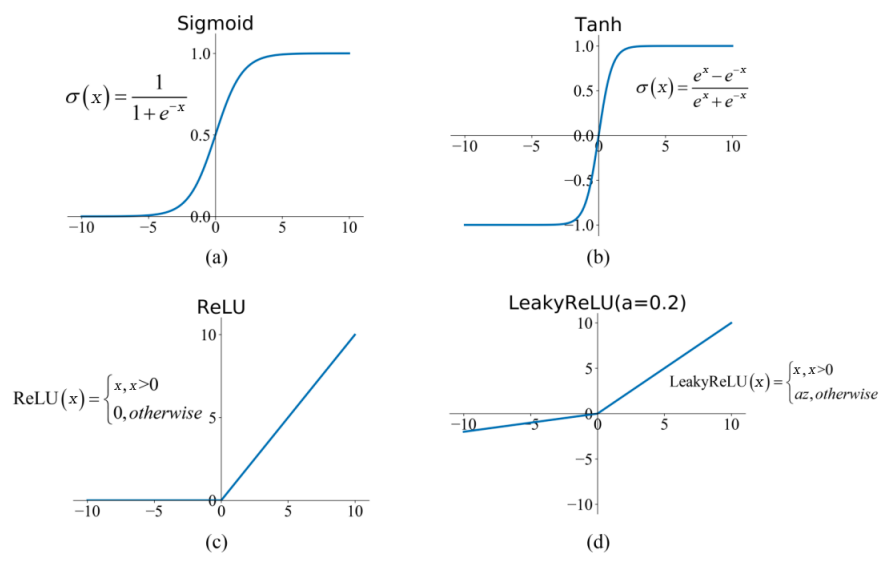
\includegraphics[width=12cm]{images_pfe/functions.png}
	\caption{Les fonctions d'activations couramment utilisées [\cite{feng_he_teng_ren_chen_li_2019}].}
	\label{fig:vue-snoc-pos}
\end{figure}
\FloatBarrier

\section{Couches dans un réseau de neurones}
Une couche (\textit{layer} en anglais) est une succession verticale des
neurones. Mathématiquement, elle est vue comme une composition de deux
fonctions \textit{h} et \textit{g} où \textit{g} est une fonction linéaire et
\textit{h} une fonction d’activation non linéaire. Cette composition de
fonction est définie par l'équation \ref{equ:couche}
[\cite{Goodfellow-et-al-2016}].

\begin{equation}
	y = h(g(x) + b)
	\label{equ:couche}
\end{equation}

\medskip
Une couche intermédiaire est donc l’ensemble des nœuds verticaux qui sont connectés à la couche précédente et à la couche suivante. La connectivité entre les couches détermine la manière dont les informations circulent sur le réseau. La façon de connexions des nœuds entre eux est différente d’une architecture à une autre [\cite{Goodfellow-et-al-2016}], et c’est ce qui détermine le type d'une couche:
\begin{itemize}
	\item \textbf{Couche entièrement connectée}: tous les neurones d'une couche sont connectés à tous les neurones de la couche suivante.
	\item \textbf{Couche partiellement connectée}: certains neurones ne sont pas connectés aux neurones de la couche suivante.
\end{itemize}

Les couches sont le composant principal des réseaux de neurones. Elles ont
plusieurs caractéristiques qui définissent leur comportement et influencent les
performances globales du réseau. Ces caractéristique sont les suivants:

\begin{itemize}
	\item \textbf{La matrice de poids}: Dans une couche d'un réseau de neurones, la matrice de poids est une matrice de paramètres qui représente les connexions entre les neurones d'entrée et les neurones de sortie de cette couche [\cite{aggarwal_2018}]. Elle définie la puissance des connexions entre les neurones des différentes couches. Chaque ligne de la matrice correspond aux poids associés à un neurone d'entrée particulier, et chaque colonne correspond aux poids associés à un neurone de sortie particulier,La taille de la matrice de poids dépend du nombre de neurones d'entrée et du nombre de neurones de sortie dans la couche.

	      La forme générale de la matrice de poids dans un réseau de neurones peut être
	      exprimée comme suit:
	      \begin{equation}
		      W = \begin{bmatrix}
			      w_{1,1} & w_{1,2} & ... & w_{1, m} \\
			      w_{2,1} & w_{2,2} & ... & w_{2, m} \\
			      ...     & ...     & ... & ...      \\
			      w_{n,1} & w_{n,2} & ... & w_{n, m}
		      \end{bmatrix}
	      \end{equation}

	      où $w_{i,j}$ représente le poids de la connexion entre le neurone \textit{i} de
	      la couche actuelle et le neurone \textit{j} de la couche suivante et
	      \textit{(n, m)} représente la dimension de la matrice.

	      La matrice de poids est crucial pour la performance du réseau neuronal,
	      puisqu'elle détermine la capacité du réseau d'apprendre et généraliser les
	      motifs a partir des données en entrées.

	\item \textbf{Type de couche}: Les couches forment les blocs de construction de base des réseaux de neurones. Elle permettent d'effectuer des calculs complexes et d'apprendre des relations qui existent entre données d'entrée et de sortie. Dans le réseau neuronal, il existe trois types de couches différents:
	      \begin{itemize}
		      \item \textbf{Couche d'entrée}: Cette couche est responsable de la réception des données d'entrée et de leur transmission à la couche suivante (la première couche parmi les couches cachées).
		      \item \textbf{Couche cachée}: Cette couche traite les entrées de la couche précédente et génère des valeurs de sortie qui sont transmises à la couche suivante. Les réseaux de neurones peuvent avoir plusieurs couches cachées, chacune effectuant différentes opérations sur les entrées.
		      \item \textbf{Couche de sortie}: Cette couche produit la sortie finale du réseau de neurones, qui peut être une classification, une régression ou un autre type de prédiction.
	      \end{itemize}
\end{itemize}

\medskip

\begin{figure}[hbt!]
	\centering
	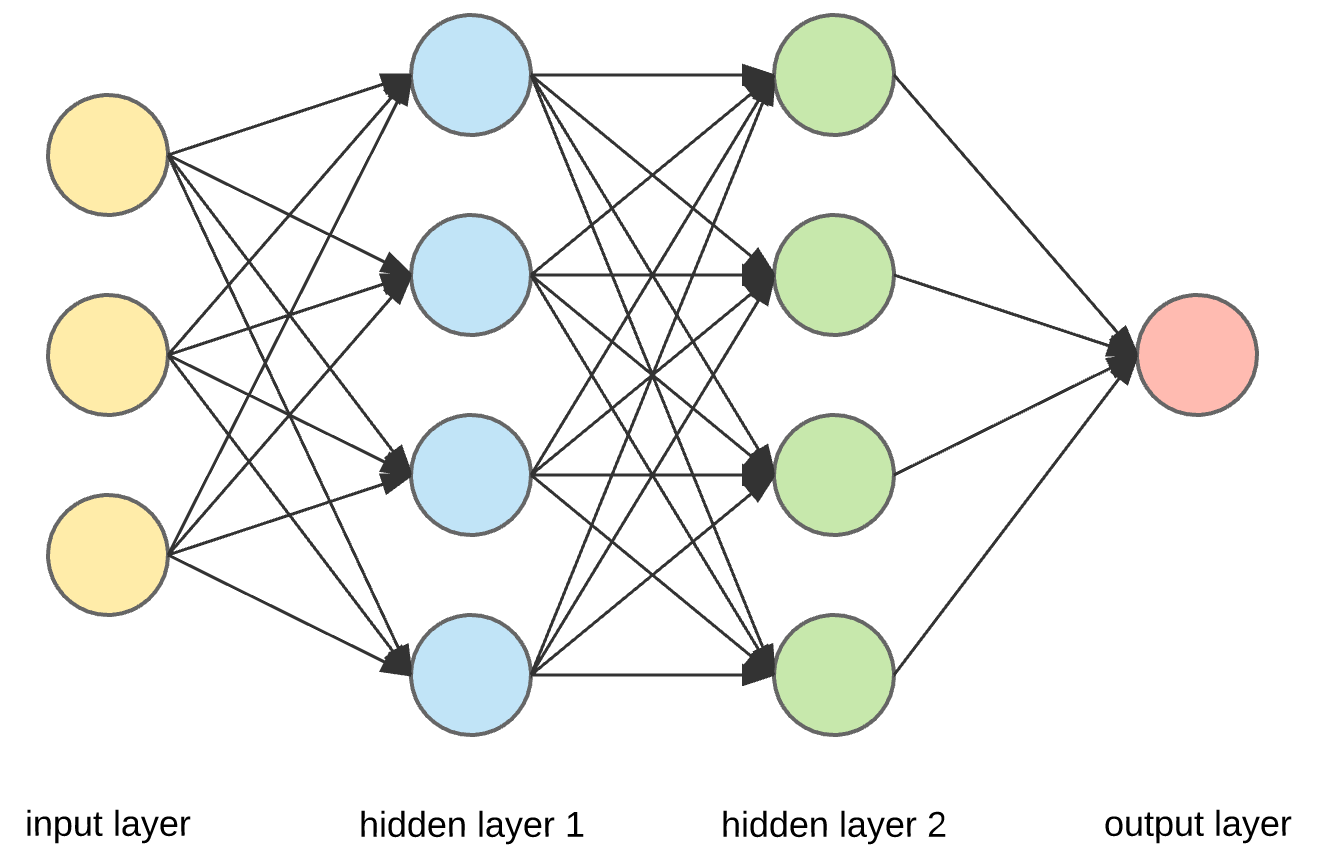
\includegraphics[width=12cm]{images_pfe/network.png}
	\caption{Schéma simple d'un réseau de neurones feedforward [\cite{dl-healthcare}].}
	\label{fig:schema-reseau}
\end{figure}
\FloatBarrier
\medskip

\section{Types de réseaux de neurones}
Dans l'apprentissage profond, il existe plusieurs classes de réseaux de
neurones, chacune avec sa propre architecture, caractéristiques, algorithme
d'apprentissage et application. Dans cette section, nous allons présenter les
différentes architecture de réseaux de neurones.
\subsection{Réseaux feedforward}
Les réseaux feedforward (ou réseaux entièrement connectés) sont un des types de
réseau de neurones artificiels où les informations circulent dans une seule
direction, de l'entrée vers la la sortie [\cite{Goodfellow-et-al-2016}]. Ils
sont composés d'une succession de couches interconnectées, où chaque neurone
d'une couche est connecté aux neurones de la couche suivante. Dans un Réseau de
ce type, les données sont introduites dans la première couche du réseau (couche
d'entrée), puis elles traversent plusieurs couches cachées avant d'atteindre la
couche de sortie (\textit{la figure \ref{fig:schema-reseau} est un schéma
	simple d'un réseau feedforward}).

Les réseaux feedforward sont indépendants de la structure, c’est-à-dire il
n’existe pas d’hypothèses particulières à faire sur l’entrée, ce qui les rend
largement applicables. Cependant, ils ont tendance à être moins performants que
les réseaux à usage spécial. Les réseaux feedforward sont couramment utilisés
dans les applications d'apprentissage supervisé. Ils peuvent également être
utilisés dans des applications d'apprentissage non supervisé
[\cite{aggarwal_2018}].

\medskip

\subsection{Réseaux de neurones récurrents (RNN)}
Les réseaux de neurones récurrents (RNN) sont des architectures conçus pour
fonctionner avec des données séquentielles, telles que: la reconnaissance de la
parole, la reconnaissance de la voie, l'analyse de séries chronologiques et le
traitement du langage naturel [\cite{Goodfellow-et-al-2016}]. Les principales
caractéristiques des RNN sont:
\begin{itemize}
	\item \textbf{Connexions récurrentes} : Les connexions dans les réseaux récurrents sont des connexions récurrentes qui permettent à l'information de persister au fil du temps. Cela signifie que la sortie du réseau à un pas de temps est réinjectée en entrée du réseau au pas de temps suivant.
	\item \textbf{État caché} : Les réseaux RNN maintiennent un état caché qui représente la mémoire du réseau. Cet état est mis à jour à chaque pas de temps en fonction de l'entrée courante et de l'état caché précédent.
	\item \textbf{RNN bidirectionnels} : Les réseaux RNN bidirectionnels traitent la séquence d'entrée dans les sens avant et arrière, ce qui permet de capturer le contexte des pas de temps passés et futurs.
\end{itemize}

\begin{figure}[hbt!]
	\centering
	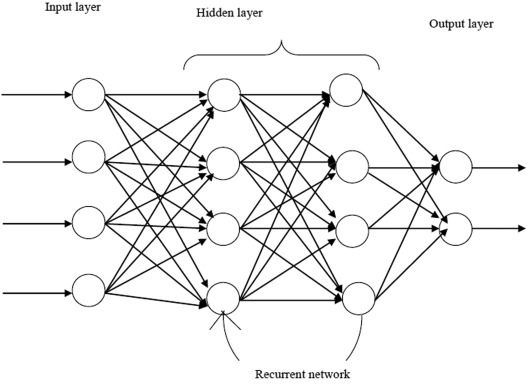
\includegraphics[width=12cm]{images_pfe/rnn.jpg}
	\caption{Exemple d'un réseau de neurones récurrent [\cite{kumaraswamy_2021}].}
	\label{fig:schema-reseau}
\end{figure}
\FloatBarrier

La capacité à conserver une mémoire des pas de temps précédents et à gérer les
dépendances à long terme rend les réseaux récurrents utiles pour les tâches qui
nécessitent de comprendre le contexte de la séquence d'entrée.

\subsection{Réseaux de neurones convolutifs (CNN)}
L'architecture des réseaus de neurones convolutifs (CNN) est une architecture
spéciale qui est bien adaptée à la tâche de classification d'images. Ces
réseaux comportent trois types de couches: \textbf{convolutives},
\textbf{pooling} et \textbf{d'activation} [\cite{Goodfellow-et-al-2016}].

Les couches convolutives sont appliquées à l'image en entrée pour l’extraction
des caractéristiques importantes de l'image. Ensuite, ces dernières traversent
des couches d'activation, qui sont responsables de l'application d'une fonction
d'activation non-linéaire à ces caractéristiques. Les couches d'activation sont
suivies de couches de pooling qui réduisent la taille de l'image. Les couches
de pooling sont elles même suivies par une couche entièrement connectée qui
donne la classification de l'image (la sortie finale du modèle)
[\cite{Goodfellow-et-al-2016}].

\begin{figure}[hbt!]
	\centering
	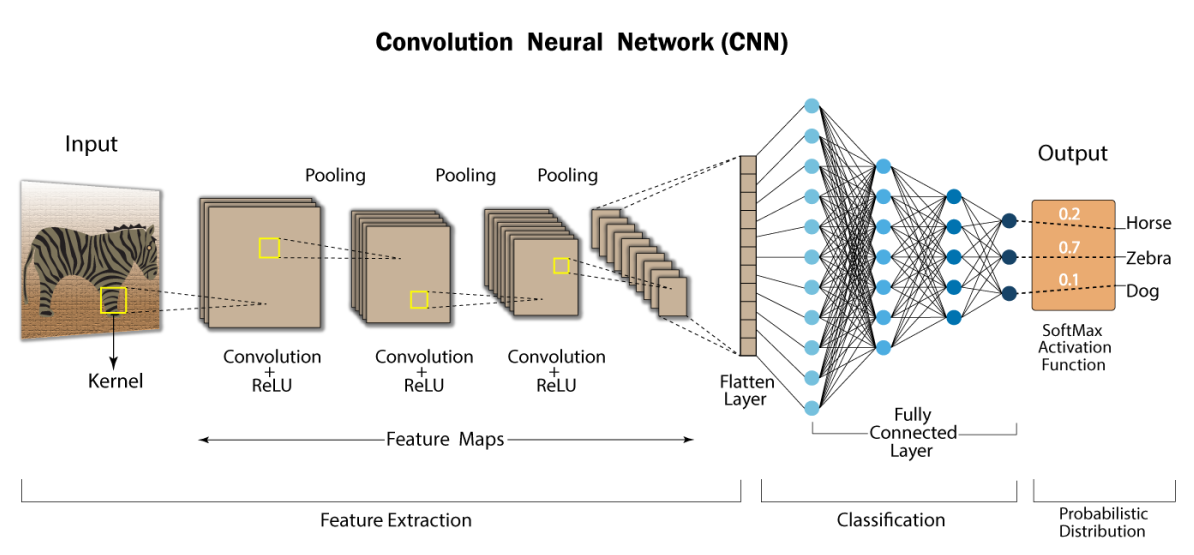
\includegraphics[width=15
		cm]{images_pfe/cnn.png}
	\caption{Le fonctionnement d'un réseau neuronal convolutif [\cite{alharbi_hewahi_2021}].}
	\label{fig:cnn}
\end{figure}
\FloatBarrier
\medskip

\subsubsection{Couche convolutive }
Une couche convolutive est un élément constitutif des réseaux de neurones
convolutifs (CNN). Elle est utilisé pour extraire des caractéristiques à partir
de données d'entrée, souvent des images, en appliquant un ensemble de filtres
convolutifs appris à l'entrée.

\medskip
Dans une couche convolutive, chaque filtre est convolué avec l'entrée pour produire une carte de caractéristiques. Cette opération est faite en glissant le filtre sur l'entrée et en calculant le produit scalaire à chaque position. Généralement, une couche convolutive possède trois hyperparamètres qui doivent être définis : \textbf{le nombre de filtres}, \textbf{la taille des filtres} et \textbf{la Stride}. Le nombre de filtres détermine le nombre de cartes d'entités produites, tandis que la taille des filtres détermine la taille du champ récepteur de chaque carte d'entités. La stride détermine la quantité de décalage du filtre à chaque étape.

\medskip
Les couches convolutives sont suivies de fonctions d'activation,et de couches de pooling. Ces dernières permettent de réduire les dimensions spatiales des cartes d'entités. Plusieurs couches convolutives peuvent être empilées pour créer un réseau neuronal convolutif profond.Les couches convolutives sont particulièrement efficaces pour traiter des images et d'autres données de grande dimension avec une structure spatiale, car elles peuvent apprendre automatiquement à détecter les caractéristiques importantes, telles que les bords, les coins et les textures [\cite{kimura_yoshinaga_sekijima_azechi_baba_2019}, \cite{Goodfellow-et-al-2016}].

\begin{figure}[hbt!]
	\centering
	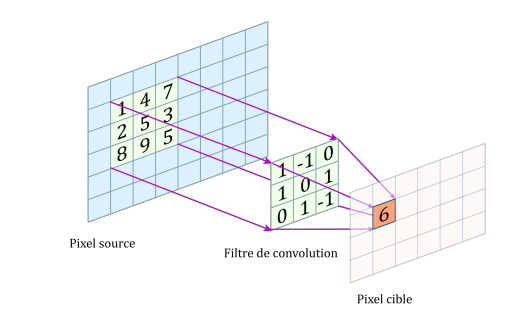
\includegraphics[width=12
		cm]{images_pfe/layerconv.png}
	\caption{Exemple du fonctionnement d'une couche convolutive [\cite{kimura_yoshinaga_sekijima_azechi_baba_2019}].}
	\label{fig:conv}
\end{figure}
\FloatBarrier
\medskip

\subsubsection{Couche pooling}
Le pooling est une opération quie est utilisée pour sous-échantillonner les
cartes de caractéristiques résultantes des couches convolutives en réduisant
leurs dimensions spatiales tout en conservant les informations importantes.
Parmi les types de pooling, on trouve le pooling maximal et le pooling moyen
	[\cite{Goodfellow-et-al-2016}].

\medskip
Dans le pooling maximal, la valeur maximale de chaque région est sélectionnée comme valeur représentative, tandis que dans le pooling moyen, la valeur moyenne est calculée à la place. Il en résulte une carte d'entités plus petite avec une résolution spatiale réduite, qui peut être traitée plus efficacement par les couches suivantes du réseau.

\medskip
Cependant, le pooling excessive peut entraîner une perte d'informations spatiales importantes. Il est donc important d'équilibrer la quantité de pooling avec les besoins du réseau et la nature de la tâche à accomplir.

\begin{figure}[hbt!]
	\centering
	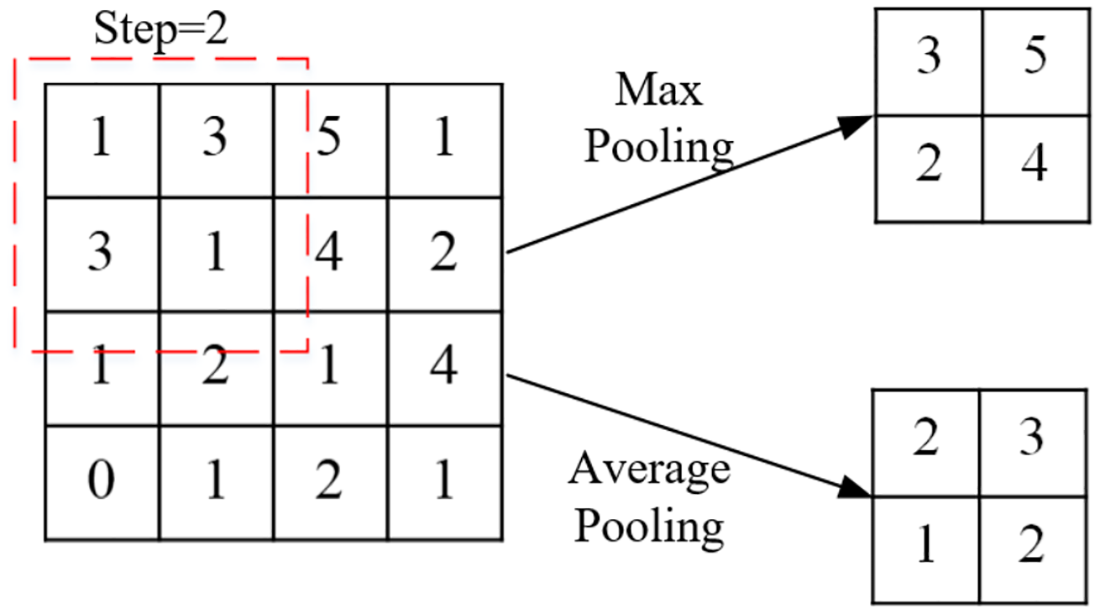
\includegraphics[width=9cm]{images_pfe/pooling.png}
	\caption{Exemples de pooling maximal et pooling moyen [\cite{hu_wu_xu_lai_xia_2022}].}
	\label{fig:pooling}
\end{figure}
\FloatBarrier
\medskip

\subsection{Réseaux générateurs adversaires (GAN)}
Les GAN (Generative Adversarial Networks) sont utilisés afin de générer des
données synthétiques, telles que des images, des vidéos ou des sons, qui
ressemblent à des données réelles. Les GAN sont composés de deux parties: le
générateur et le discriminant
	[\cite{goodfellow_pouget-abadie_mirza_xu_warde-farley_ozair_courville_bengio_2020}].

\medskip
Le générateur prend comme entrée un vecteur de bruit aléatoire et produit en sortie une image synthétique, tandis que le discriminant en entrée prend une image et produit en sortie une probabilité qui indique si l'image est réelle ou synthétique. Les deux réseaux sont formés en même temps, avec le générateur essayant de tromper le discriminant en produisant des images synthétiques qui sont indiscernables des images réelles [\cite{goodfellow_pouget-abadie_mirza_xu_warde-farley_ozair_courville_bengio_2020}, \cite{feng_feng_chen_cao_zhang_jiao_yu_2020}].

\medskip
Les GAN sont capables de produire des résultats très proches des données réelles, allant de portraits d'humains à des paysages naturels, en passant par des objets et des bâtiments. Cependant, ils sont souvent difficiles à former et peuvent être instables, en particulier lorsque les données d'entrée sont complexes.

\begin{figure}[hbt!]
	\centering
	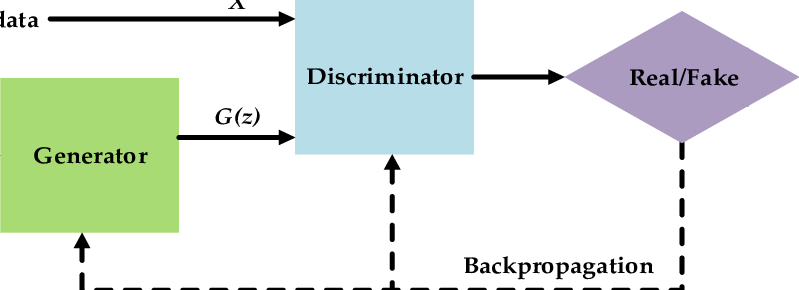
\includegraphics[width=12cm]{images_pfe/gan.png}
	\caption{Un modèle de réseau générateur adversaire (GAN) [\cite{feng_feng_chen_cao_zhang_jiao_yu_2020}].}
	\label{fig:gan}
\end{figure}
\FloatBarrier

\subsection{Réseaux de neurones de transformation (Transformer)}
Les réseaux de neurones de transformation (Transformers) sont une architecture
de réseau de neurones conçue par Google. Il sont utilises principalement pour
le traitement du langage naturel, la traduction du texte et la génération de
texte.

\medskip
De ce fait, les Transformers ressemblent aux réseaux récurrents (RNN) mais la principale différence entre eux est que les Transformers n'utilisent pas de couches récurrentes pour modéliser les dépendances séquentielles. Au lieu de cela, ils utilisent une technique appelée "self-attention", qui permet au modèle de s'auto-atténuer sur les parties importantes de l'entrée [\cite{attention_is_all_you_need}].

\medskip
Dans un réseau de neurones à auto-attention, chaque mot ou token en entrée est représenté par un vecteur, et ces vecteurs sont utilisés pour calculer les scores d'attention entre les différentes parties de l'entrée. Ces scores sont ensuite utilisés pour pondérer les vecteurs en entrée, en mettant plus d'importance sur les parties les plus pertinentes [\cite{attention_is_all_you_need}].

\medskip
Les Transformers ont contribué significativement aux avancées récentes dans le domaine du traitement du langage naturel, en particulier dans la traduction automatique et de la génération de texte. Les modèles les plus avancés, telles que GPT-3 de OpenAI ou Bard de Google, utilisent des architectures de Transformers massives avec des milliards de paramètres.

\begin{figure}[hbt!]
	\centering
	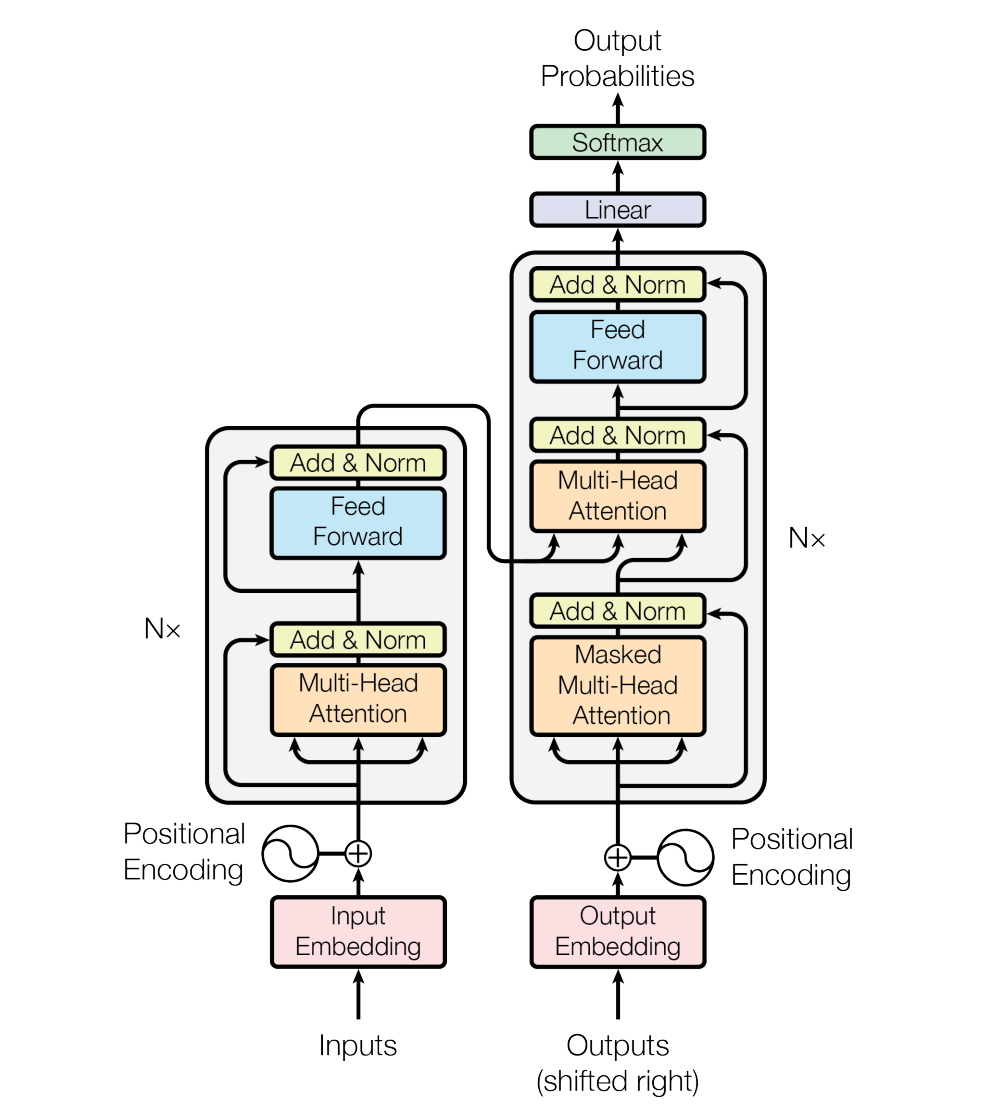
\includegraphics[width=12cm]{images_pfe/transformer-architecture.png}
	\caption{Architecture d'un reseau de neurones de transformation (Transformer) [\cite{attention_is_all_you_need}].}
	\label{fig:gan}
\end{figure}
\FloatBarrier

\subsection{Réseaux résiduels (ResNet)}
Les réseaux résiduels ont été conçus par Microsoft afin de résoudre le problème
des gradients qui disparaissent dans les réseaux de neurones très profonds, ce
qui peut rendre l'entraînement difficile et diminuer significativement les
performances du réseau.

\medskip
Un ResNet est composé d'une ensemble de blocs résiduels, qui sont constitués de plusieurs couches avec des connexions de raccourci qui contournent une ou plusieurs couches. Ces raccourcis permettent aux gradients de circuler plus facilement à travers le réseau et évitent qu'ils ne disparaissent à mesure que le réseau devient plus profond [\cite{He_2016_CVPR}].

\begin{figure}[hbt!]
	\centering
	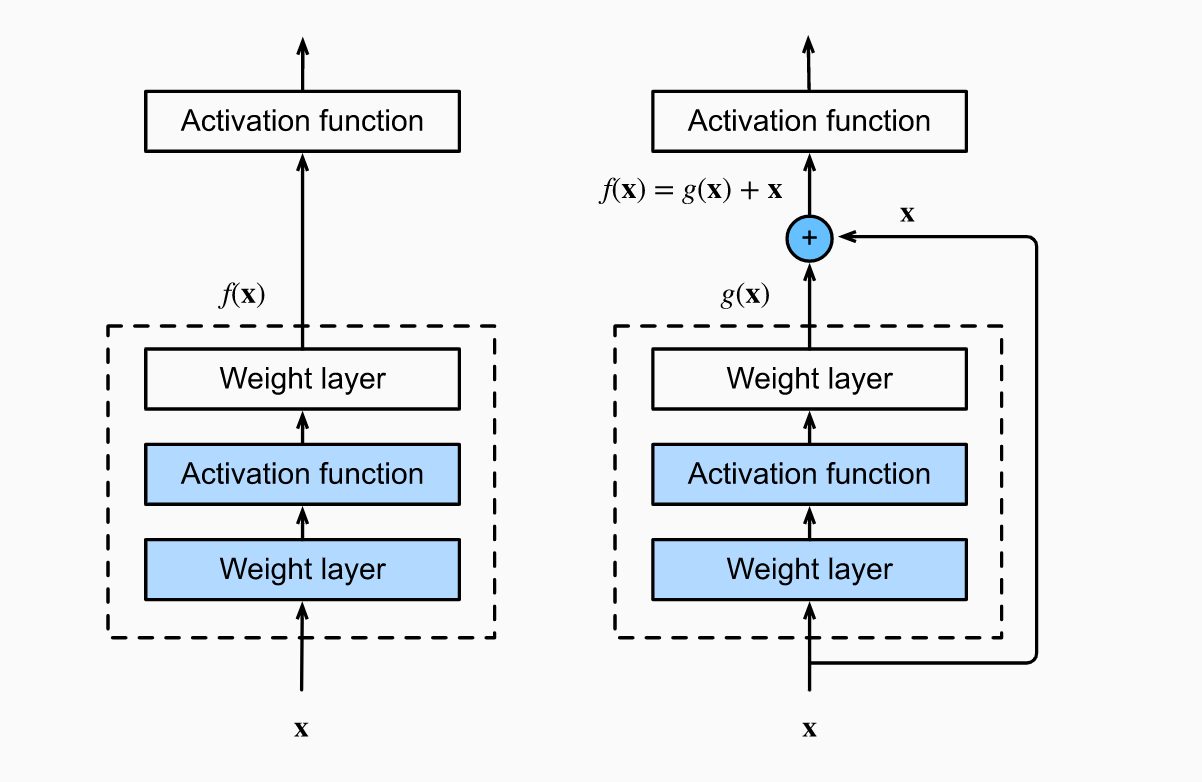
\includegraphics[width=12cm]{images_pfe/residual-net.png}
	\caption{Un bloc régulier (gauche) et un bloc résiduel (droite) [\cite{dong_niu_li_xie_zou_ye_wei_pan_2022}].}
	\label{fig:residual-net}
\end{figure}
\FloatBarrier

\medskip
ResNet est très efficace dans les tâches de vision par ordinateur, telles que la classification d'images, la détection d'objets et la segmentation. Il a joué un rôle important dans l'avancement de l'état de l'art en apprentissage profond et en vision par ordinateur, et continue d'être un domaine de recherche actif.

\subsection{Réseaux de neurones en graphe (GNN)}
Les réseaux de neurones en graphe (GNN) sont conçus pour traiter des données
structurées sous forme de graphes. Les GNN sont capables d'apprendre et de
faire des prédictions sur les données du graphe en propageant les informations
à travers les bords et les nœuds du graphe [\cite{ZHOU202057}].

\medskip
L'idée de base derrière les GNN est d'utiliser un ensemble de paramètres entraînables pour transformer les caractéristiques de chaque nœud dans le graphe en fonction des caractéristiques de ses nœuds voisins (plongement de graphe). Ce processus est répété de manière itérative sur plusieurs couches du réseau, permettant au GNN d'apprendre des motifs et des relations complexes à partir des données [\cite{ZHOU202057}].

\medskip
Parmi les tâches réalisées par ce type de réseaux:
\begin{itemize}
	\item \textbf{Classification des graphes} : Les GNN peuvent être utilisées pour classer des graphes en différentes catégories, tels que dans le cas de l'analyse des réseaux sociaux, la classification de textes et classification des molécules.
	\item \textbf{Prédiction de lien} : Les GNN peuvent prédire le lien manquant entre une paire de nœuds dans un graphe avec une matrice d'adjacence incomplète. Ils sont souvent utilisés pour les réseaux sociaux (tel que la suggestion des amis)
	\item \textbf{Plongement de graphe} : Les GNN permettent de faire la transformation de graphe en vecteurs, en préservant les informations pertinentes sur les nœuds, les arêtes et la structure générale du graphe.
\end{itemize}

\begin{figure}[hbt!]
	\centering
	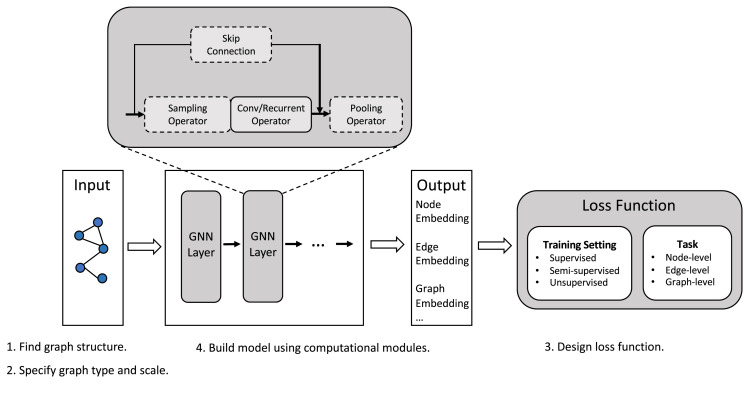
\includegraphics[width=15cm]{images_pfe/gnn.jpg}
	\caption{Le pipeline de conception générale pour un modèle GNN [\cite{ZHOU202057}].}
	\label{fig:gnn}
\end{figure}
\FloatBarrier
\medskip

\section{Le processus d’apprentissage}
L’apprentissage est le processus itératif et continu d’ajustement des
paramètres du réseau neuronal afin d’obtenir une meilleure précision du modèle
[\cite{Goodfellow-et-al-2016}]. Il peut être complexe car il nécessite souvent
une combinaison de techniques telles que le \textbf{prétraitement} des données,
le choix de l'architecture du réseau de neurones et des hyperparamètres, ainsi
que l'algorithme d'optimisation.

Ce processus d'apprentissage commence d'abord par l'initialisation aléatoire
des paramètres (poids) du modèle. Ensuite, le modèle est entraîné sur un
ensemble de données (\textbf{dataset}) en utilisant un algorithme
d'optimisation pour ajuster les poids du modèle afin de minimiser la perte.

Lors de l'entraînement, le modèle est alimenté en entrée avec des exemples à
partir du dataset d'entrainement et compare sa sortie à la sortie attendue.
Ensuite, il calcul la perte en faisant la différence entre la sortie prédite et
la sortie attendue. L'algorithme de \textbf{rétropropagation} de gradient
ajuste les poids du modèle en claculant les gradient de la fonction de perte
afin de la minimiser.

Le processus d'apprentissage continue jusqu'à ce que la performance du modèle
sur le dataset de validation arrête de s'améliorer ou jusqu'à ce qu'un nombre
prédéfini d'itérations d'apprentissage soit atteint. Le modèle final est
ensuite utilisé pour effectuer des prédictions sur de nouvelles données.

\medskip
Ce processus peut être résumé dans les points suivants:
\begin{itemize}
	\item L’apprentissage consiste à modifier progressivement les paramètres (poids) en
	      passant un lot de données en entrée et en évaluant le taux de perte.
	\item La définition de la fonction de perte est utilisée pour les modifications de
	      réseaux dans le processus de l'entraînement.
	\item La modification des poids du réseau est effectuée grâce a l’algorithme de
	      rétropropagation (backpropagation).
\end{itemize}

\subsection{Descente de gradient}
La descente de gradient est une méthode utilisée dans le processus
d’optimisation. Elle est basée sur la différentiabilité d’une fonction et elle
est appliquée pour calculer la fonction dérivée du premier ordre pour trouver
le minimum de la fonction de perte [\cite{Goodfellow-et-al-2016}]. Sa
simplicité d’application est l’un des avantages de cette méthode.

L'algorithme commence par l'initialisation aléatoire des paramètres (poids) du
modèle. Ensuite, il calcule le gradient de la fonction de perte par rapport à
chaque paramètre. Le gradient indique la direction dans laquelle la fonction de
perte augmente le plus, donc l'algorithme met à jour les paramètres dans la
direction opposée au gradient pour réduire la valeur de perte. Ce processus est
répété itérativement jusqu'à ce que la valeur de perte ne puisse plus être
réduite ou jusqu'à ce qu'un critère d'arrêt soit atteint. Le taux
d'apprentissage est un hyperparamètre qui contrôle la taille des mises à jour
de paramètres et la vitesse de convergence de l'algorithme
[\cite{Goodfellow-et-al-2016}].

Des variantes de la descente de gradient existent, telles que la descente de
gradient stochastique, Adam et la descente de gradient avec moment.

\subsection{Propagation de l’erreur}
La propagation d'erreur est utilisée dans le processus d'apprentissage pour
calculer le gradient de la fonction de perte par rapport aux paramètres du
modèle [\cite{Goodfellow-et-al-2016}].

Dans la propagation d'erreur, l'erreur est propagée en arrière à travers les
couches du modèle, en commençant par la couche de sortie et en allant vers
l'entrée. Chaque couche calcule la dérivée de sa sortie par rapport à ses
entrées, qui est ensuite multipliée par l'erreur propagée de la couche
suivante. Ce processus est répété jusqu'à ce que l'erreur soit propagée jusqu'à
la couche d'entrée, où le gradient de la fonction de perte par rapport aux
paramètres du modèle est obtenu [\cite{Goodfellow-et-al-2016}].

\begin{figure}[hbt!]
	\centering
	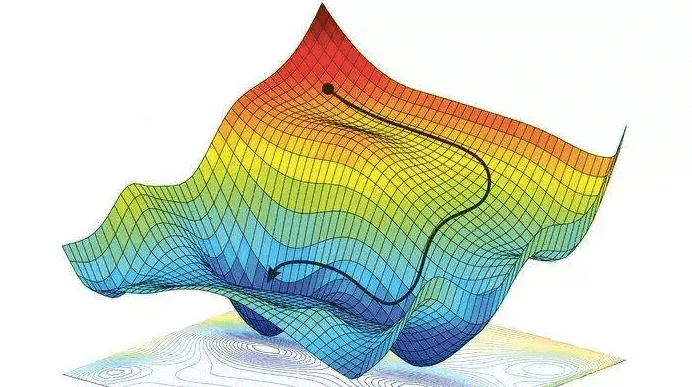
\includegraphics[width=10cm]{images_pfe/gd.png}
	\caption{Fonction de taux d’erreur [\cite{amini2018spatial}].}
	\label{fig:error-function}
\end{figure}
\FloatBarrier
\medskip

\subsection{Hyperparameters}
Les hyperparamètres sont les paramètres qui sont définis avant de lancer le
processus d'apprentissage et ils contrôlent l'entraînement. Les valeurs des
hyperparamètres, contrairement aux paramètres du modèle, ne sont pas apprises
lors de l'apprentissage [\cite{Goodfellow-et-al-2016}]. Parmi les
hyperparamètres, on peut définir:
\begin{itemize}
	\item \textbf{Taux d'apprentissage} : Il contrôle la vitesse d'apprentissage du modèle à partir des données.
	\item \textbf{Nombre d'époques} : Le nombre d'époques correspond au nombre d'itération sur le dataset d'entraînement.
	\item \textbf{Taille du batch} : Elle représente le nombre d'échantillons des données d'entraînement qui sont utilisés dans un passage avant/arrière (feedforward et backpropagation).
	\item \textbf{Nombre de couches} : C'est un hyperparamètre qui caractérise la profondeur du réseau.
	\item \textbf{Fonction d'activation} : La fonction d'activation est utilisée pour introduire la non-linéarité dans le modèle. C'est un hyperparamètre qui contrôle la sortie du neurone.
	\item \textbf{Initialisation des poids} : Les valeurs initiales des poids peuvent affecter de manière significative les performances du modèle. Elle affecte le processus de trouver le minimum local ou le minimum global.
	\item \textbf{Paramètre de régularisation} : Il est utilisé pour éviter le \textbf{surapprentissage}, c'est-à-dire éviter de construire un modèle qui est trop complexe par rapport à la quantité de données d'entraînement. Cela peut entraîner une adaptation excessive du modèle aux données d'entraînement et une mauvaise généralisation aux données inconnues.
	\item \textbf{Optimiseur} : L'optimiseur est l'algorithme utilisé pour mettre à jour les poids pendant l'entraînement.
\end{itemize}

Cependant, le réglage de ces hyperparamètres peut être une tâche complexe
nécessitant souvent des essais et des erreurs.

\section{Types d’apprentissage}
Il existe plusieurs types d’apprentissage, et chacun de ces types a des
applications spécifiques en deep learning, et peut être utilisé pour résoudre
différents types de problèmes. Dans ce qui suit, nous parlons brièvement sur
les quatre types d'apprentissage en deep learning les plus courants:
l'apprentissage supervisé, l'apprentissage non supervisé, l'apprentissage
semi-supervisé et l'apprentissage par renforcement.

\subsection{Apprentissage supervisé}
Dans l'apprentissage supervisé, l'apprentissage s'effectue sur un ensemble de
données étiqueté, où les étiquettes sont connues à l'avance. En d'autres
termes, les données d'entrée sont accompagnées d'étiquettes de sortie ou de
valeurs cibles correspondantes. Le but de l'apprentissage supervisé est
d'apprendre à prédire les étiquettes à partir des données d'entrée, de sorte
que lorsqu'on donne au modèle de nouvelles données en entrée, l'algorithme
puisse prédire la sortie correspondante. Pendant le processus d'apprentissage,
l'algorithme ajuste itérativement ses paramètres pour minimiser la différence
entre la sortie prédite et la sortie réelle [\cite{aggarwal_2018},
\cite{Goodfellow-et-al-2016}].

\medskip
Ce type d'apprentissage est applicable dans plusieurs domaines, tels que la reconnaissance d'images et de la parole, le traitement du langage naturel et la modélisation prédictive dans la finance, la santé, le marketing, etc. Parmi les algorithmes d'apprentissage supervisés, nous pouvons citer la régression linéaire et les arbres de décision.

\subsection{Apprentissage non-supervisé}
L'apprentissage non supervisé se fait sur un dataset non étiqueté, sans aucune
information sur les étiquettes [\cite{Goodfellow-et-al-2016}]. En d'autres
termes, il n'y a pas de valeurs cibles ou d'étiquettes de sortie fournies à
l'algorithme. L'algorithme est laissé à lui-même pour trouver les motifs et
relations dans les données, sans recevoir d'instructions explicites sur ce
qu'il faut rechercher.

\medskip
L'utilisation de cette approche d'apprentissage peut impliquer le regroupement de points de données similaires, la découverte de structures ou de caractéristiques cachées dans les données (réduction de la dimensionnalité) ou l'identification de valeurs aberrantes ou d'anomalies dans les données.

\medskip
Nous pouvons appliquer l'apprentissage non supervisé dans divers domaines, tels que la segmentation des marchés, la détection d'anomalies et l'extraction de caractéristiques. Parmi les algorithmes d'apprentissage non supervisés courants, on trouve le clustering k-means, l'analyse en composantes principales (PCA) et les auto-encodeurs.

\medskip
L'un des principaux défis dans l'apprentissage non supervisé est d'évaluer la qualité des résultats, car il n'y a pas d'objectifs ou d'étiquettes explicites à comparer. Au lieu de cela, les résultats sont souvent évalués en fonction de leur utilité ou de leur interprétabilité pour une tâche ou un domaine particulier.

\subsection{Apprentissage semi-supervisé}
L'apprentissage semi-supervisé est un type d'apprentissage qui combine des
éléments d'apprentissage supervisé et non supervisé. Dans l'apprentissage
semi-supervisé, un petit ensemble de données étiquetées est fourni, tandis que
la grande partie de données est non étiquetées [\cite{Goodfellow-et-al-2016}].

\medskip
Le but dans l'apprentissage semi-supervisé est d'utiliser les données étiquetées pour guider le processus d'apprentissage sur les données non étiquetées, afin d'améliorer la précision du modèle. Cela peut être particulièrement utile dans les situations où il est difficile ou coûteux d'obtenir des données étiquetées, mais il existe une abondance de données non étiquetées disponibles.

\medskip
Il existe plusieurs approches, mais une méthode courante consiste à utiliser les données étiquetées pour créer un modèle, puis à utiliser ce modèle pour faire des prédictions sur les données non étiquetées. Les étiquettes prédites sont ensuite utilisées pour améliorer le modèle, et le processus est répété de manière itérative.

\medskip
L'un des défis de l'apprentissage semi-supervisé est que la qualité des résultats peut dépendre fortement de la distribution des données non étiquetées. Si les données non étiquetées ne sont pas représentatives du domaine cible, le modèle peut mal fonctionner même avec une grande quantité de données non étiquetées.

\subsection{Apprentissage par renforcement}
L'apprentissage par renforcement se concentre sur la prise de décision. Il
s'agit d'une méthode d'apprentissage dans laquelle un agent apprend à prendre
des décisions en interagissant avec un environnement. L'agent doit choisir une
action à partir d'un état donné, et l'environnement renvoie un signal de
récompense ou de pénalité en fonction de l'action choisie. L'objectif de
l'agent est de maximiser la récompense totale sur une période donnée
[\cite{wiering2012reinforcement}]. Dans le chapitre suivant, nous présenterons
l'apprentissage par renforcement et nous en parlerons avec plus de détails.

\section{Catégories de données}
La division du jeu de données est une étape cruciale avant de commencer
l'entraînement du modèle de manière. Elle permet d'éviter les problèmes de
surapprentissage. Il est courant de diviser un jeu de données en trois parties
distinctes: l'ensemble d'entraînement, l'ensemble de validation et l'ensemble
de test [\cite{Goodfellow-et-al-2016}].

\begin{itemize}
	\item \textbf{Ensemble d'entraînement}: Il s'agit de la partie de données utilisée pour entraîner le modèle. Il est important que ce dataset soit représentatif de l'ensemble des données et qu'il contienne une variété de cas d'utilisation différents.

	\item \textbf{Ensemble de validation}: Il s'agit d'un sous-ensemble de l'ensemble de données utilisé pour évaluer les performances du modèle pendant l'entraînement. L'ensemble de validation est utilisé pour régler les hyperparamètres du modèle et pour éviter le surapprentissage. Il est important qu'il soit représentatif et distinct du dataset d'entraînement.

	\item \textbf{Ensemble de test}: Il s'agit d'un ensemble de données utilisé pour évaluer les performances du modèle après son entraînement. L'ensemble de test est utilisé pour obtenir une estimation impartiale de la performance du modèle sur de nouvelles données inédites, donc il est nécessaire que ce dataset soit représentatif de l'ensemble des données et distinct des deux autres datasets cités précédemment.
\end{itemize}
La distinctivité des datasets assure que le modèle se généralise bien aux nouvelles données invisibles. En règle générale, l'ensemble de données est divisé en ces trois ensembles dans un rapport de 60-20-20 ou 70-15-15 respectivement.

\section{Défis de l'apprentissage profond}
L'apprentissage profond a fait des progrès remarquables ces dernières années et
a obtenu des résultats excellents dans divers domaines tels que la vision par
ordinateur, le traitement du langage naturel et la reconnaissance de la parole.
Cependant, il reste encore plusieurs défis à relever afin d'améliorer encore
l'efficacité et l'efficience des modèles d'apprentissage profond. Certains
défis majeurs incluent:
\begin{itemize}
	\item \textbf{Rareté des données} : les modèles d'apprentissage profond nécessitent une grande quantité de données pour être entraînés efficacement. Cependant, dans de nombreux domaines, tels que l'imagerie médicale et la conduite autonome, les données sont rares et coûteuses à collecter.

	\item \textbf{Surapprentissage (overfitting)} : les modèles d'apprentissage profond peuvent facilement sur-adapter les données d'apprentissage, en particulier lorsque le modèle comporte un grand nombre de paramètres. Le surapprentissage peut entraîner de mauvaises performances de généralisation sur de nouvelles données.

	\item \textbf{Interprétabilité} : les modèles d'apprentissage profond sont souvent appelés "boîtes noires" car il peut être difficile de comprendre comment ils arrivent à leurs prédictions. Ce manque d'interprétabilité peut compliquer le débogage et l'amélioration des modèles de l’apprentissage profond

	\item \textbf{Limitations matérielles} : les modèles d'apprentissage profond  sont coûteux en termes de calcul et nécessitent un matériel spécialisé tel que des unités de traitement graphique (GPU) ou des unités de traitement de tenseur (TPU). Le coût de ce matériel peut constituer un obstacle pour les petits groupes de chercheurs ou les entreprises.

	\item \textbf{Attaques contradictoires} : les modèles d'apprentissage profond  peuvent être vulnérables aux attaques contradictoires, où un attaquant manipule délibérément les données d'entrée pour amener le modèle à faire des prédictions incorrectes.

\end{itemize}

\section{Conclusion}
En conclusion, l'apprentissage profond est devenu un domaine de recherche actif
de l'apprentissage automatique qui a révolutionné la façon dont nous abordons
de nombreux problèmes difficiles, tels que la vision par ordinateur, le
traitement du langage naturel et la robotique. Avec l'avènement d'un matériel
puissant, d'ensembles de données à grande échelle et d'algorithmes
sophistiqués, les modèles d'apprentissage profond ont connu un avancement
remarquable dans plusieurs domaines tels que la reconnaissance d'images, la
reconnaissance vocale, la traduction linguistique et la conduite autonome.

\medskip
Malgré son énorme succès, l'apprentissage en profondeur fait encore face à plusieurs défis, tels que le besoin d'algorithmes d'entraînement plus efficaces et fiables, une meilleure interprétabilité, etc. L’utilisation et l'entraînement de modèles d’apprentissage profond exigent des ordinateurs assez puissants et ne peuvent pas être utilisés sur les appareils moins puissants comme les ordinateur embarqués ou les smartphones, ce qui signifie qu'on a besoin de trouver des moyens pour optimisation ces modèles afin de les utiliser ultérieurement par les machines moins puissantes. Ces méthodes d'optimisation font l'objet du dernier chapitre.

\medskip
Dans ce qui suit, nous présenterons l'apprentissage profond et ses algorithmes. La raison pour laquelle on a réservé un chapitre complet pour l'apprentissage profond est que ce type d'apprentissage peut aider beaucoup dans l'optimisation des réseaux de neurones profonds, comme nous le verrons plus tard.

\clearpage




%%%%%%%%%%%%%%%%%%%%%%%%%%%%%% Intelligence artificielle générative (GenAI) %%%%%%%%%%%%%%%%%%%%%%%%%%%%%%%%%%%%%%%


\chapter{Intelligence Artificielle Générative (GenAI)}
\section{Introduction}

Avec les avancées fulgurantes du deep learning, de nouvelles méthodes
d'intelligence artificielle ont émergé, souvent désignées sous le terme de
modèles génératifs. Ces technologies de pointe, telles que les auto-encodeurs
variationnels, les réseaux adversariaux génératifs (GAN), les modèles de
diffusion, les transformers et les modèles de langage de grande taille (LLM)
sont capables de produire des données d'une qualité impressionnante,
ressemblant de manière frappante aux données réelles. Les données générées par
ces modèles sont souvent indiscernables des données authentiques, ce qui pose
de nouveaux défis en matière d'identification et d'authenticité.Les modèles
génératifs permettent la génération de textes, d'images, de séries temporelles
et de données tabulaires avec une grande précision.

\medskip

La puissance de ces modèles repose sur des ressources de calcul considérables,
notamment l'utilisation de GPU, et sur l'accès à des ensembles de données
massifs. Par exemple, des modèles tels que ChatGPT-4 ont été entraînés sur
l'intégralité du contenu disponible sur Internet.

\medskip

Dans ce chapitre, nous allons examiner en détail les différentes architectures
de ces modèles génératifs, ainsi que les techniques et pratiques associées à
leur fonctionnement et à leur mise en œuvre. Nous aborderons les principes de
base, les innovations récentes, et les applications potentielles de ces
technologies révolutionnaires.



\section{Les Auto-Encodeurs Variationnels (VAE)}
\subsection{Introduction}

Les auto-encodeurs variationnels (VAE) sont des modèles génératifs puissants, reconnus pour leur capacité à
apprendre une représentation compacte et structurée des données. Cette approche a révolutionné le domaine de
l'apprentissage non supervisé et des modèles génératifs. Les VAE appartiennent à la classe des modèles génératifs
probabilistes, combinant les principes des autoencodeurs et des modèles de variational Bayes pour générer des 
données nouvelles et similaires à celles d'un jeu de données d'entraînement. 
Depuis leur introduction par Kingma et Welling en 2013 [\cite{kingma_welling_auto_encoding}] , les VAE ont connu un grand succès dans diverses applications, allant de la génération d'images à la synthèse de texte.



\subsection{Fonctionnement}
\textbf{L'Encodeur:}L'encodeur est responsable de la transformation des données d'entrée \(\mathbf{x}\) en une distribution 
dans l'espace latent. Plus précisément, il mappe les données d'entrée à une distribution gaussienne paramétrée par 
une moyenne \(\mu\) et une variance \(\sigma^2\). Cette distribution est souvent représentée comme :


\begin{equation}
	q(\mathbf{z} \mid \mathbf{x}) = \mathcal{N}(\mathbf{z} \mid \mu(\mathbf{x}), \sigma^2(\mathbf{x}))
	\label{equ:couche}
\end{equation}


où \(\mathbf{z}\) est la variable latente que l'encodeur cherche à estimer.

\medskip

\textbf{Le Décodeur:}Le décodeur prend un échantillon \(\mathbf{z}\) de la distribution gaussienne dans
l'espace latent et génère une reconstruction \(\hat{\mathbf{x}}\) des données d'entrée. Il modélise la distribution
 des données d'entrée conditionnellement à \(\mathbf{z}\) comme suit :



\begin{equation}
	p(\mathbf{x} \mid \mathbf{z})
	\label{equ:couche}
\end{equation}


Typiquement, le décodeur est un réseau neuronal qui produit les paramètres de cette distribution, 
souvent supposée gaussienne ou Bernoulli selon la nature des données.

\medskip

\textbf{L'Espace latent:}est la représentation comprimée et structurée des données d'entrée. 
Il est généralement conçu comme un espace continu, où chaque point de l'espace latent correspond à une instance
possible de données générées. L'idée est que cet espace latent capture les caractéristiques essentielles 
des données d'entrée de manière à permettre 
la génération de nouvelles instances en échantillonnant de cet espace.

\begin{figure}[hbt!]
	\centering
	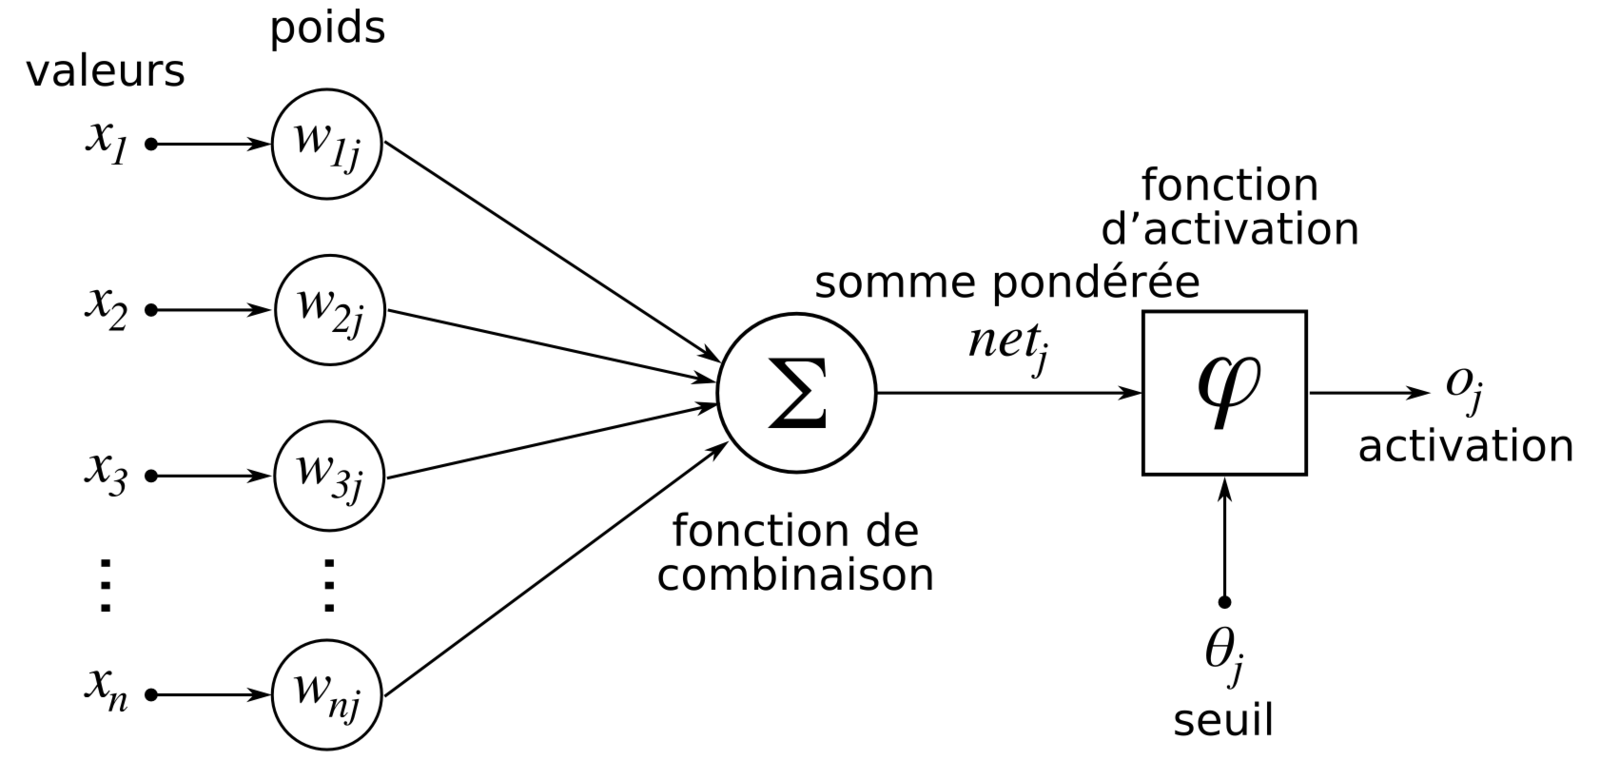
\includegraphics[width=10cm]{images_pfe/neurone.png}
	\caption{Le fonctionnement d'un neurone artificiel [\cite{mcculloch_pitts_1943_nervous_activity}].}
	\label{fig:fonctionnement-neurone}
\end{figure}


\textbf{Fonction de Coût: }l'objectif d'un VAE est d'optimiser la fonction de coût qui combine deux termes principaux : la divergence de Kullback-Leibler (KL) entre la distribution latente approximée \( q(\mathbf{z} \mid \mathbf{x}) \) et la distribution prior \( p(\mathbf{z}) \), et la vraisemblance de reconstruction \( p(\mathbf{x} \mid \mathbf{z}) \). La fonction de coût totale, appelée la fonction de perte VAE, est donnée par :

\[
\mathcal{L}(\mathbf{x}; \theta, \phi) = \text{KL}\left[q(\mathbf{z} \mid \mathbf{x}) \parallel p(\mathbf{z})\right] - \mathbb{E}_{q(\mathbf{z} \mid \mathbf{x})}[\log p(\mathbf{x} \mid \mathbf{z})]
\]

où :

\[
\text{KL}\left[q(\mathbf{z} \mid \mathbf{x}) \parallel p(\mathbf{z})\right]
\]

mesure la divergence entre la distribution latente approximée et la distribution prior.

\[
\mathbb{E}_{q(\mathbf{z} \mid \mathbf{x})}[\log p(\mathbf{x} \mid \mathbf{z})]
\]

est l'espérance de la log-vraisemblance de la reconstruction des données données la variable latente.

L'optimisation de cette fonction de coût permet au VAE d'apprendre à générer des données qui ressemblent aux données d'entrée tout en apprenant une représentation efficace dans l'espace latent.
```